\documentclass[12pt]{extarticle}

\usepackage{multicol}

% Document Layout and Font
\usepackage{subfiles}
\usepackage[margin=2cm, headheight=15pt]{geometry}
\usepackage{fancyhdr}
\usepackage{enumitem}	
\usepackage{wrapfig}
\usepackage{float}
\usepackage{multicol}

\usepackage[p,osf]{scholax}

\renewcommand*\contentsname{Table of Contents}
\renewcommand{\headrulewidth}{0pt}
\pagestyle{fancy}
\fancyhf{}
\fancyfoot[R]{$\thepage$}
\setlength{\parindent}{0cm}
\setlength{\headheight}{17pt}
\hfuzz=9pt

% Figures
\usepackage{svg}

% Utility Management
\usepackage{color}
\usepackage{colortbl}
\usepackage{xcolor}
\usepackage{xpatch}
\usepackage{xparse}

\definecolor{gBlue}{HTML}{7daea3}
\definecolor{gOrange}{HTML}{e78a4e}
\definecolor{gGreen}{HTML}{a9b665}
\definecolor{gPurple}{HTML}{d3869b}

\definecolor{links}{HTML}{1c73a5}
\definecolor{bar}{HTML}{584AA8}

% Math Packages
\usepackage{mathtools, amsmath, amsthm, thmtools, amssymb, physics}
\usepackage[scaled=1.075,ncf,vvarbb]{newtxmath}

\newcommand\B{\mathbb{C}}
\newcommand\C{\mathbb{C}}
\newcommand\R{\mathbb{R}}
\newcommand\Q{\mathbb{Q}}
\newcommand\N{\mathbb{N}}
\newcommand\Z{\mathbb{Z}}

\DeclareMathOperator{\lcm}{lcm}

% Probability Theory
\newcommand\Prob[1]{\mathbb{P}\qty(#1)}
\newcommand\Var[1]{\text{Var}\qty(#1)}
\newcommand\Exp[1]{\mathbb{E}\qty[#1]}

% Analysis
\newcommand\ball[1]{\B\qty(#1)}
\newcommand\conj[1]{\overline{#1}}
\DeclareMathOperator{\Arg}{Arg}
\DeclareMathOperator{\cis}{cis}

% Linear Algebra
\DeclareMathOperator{\dom}{dom}
\DeclareMathOperator{\range}{range}
\DeclareMathOperator{\spann}{span}
\DeclareMathOperator{\nullity}{nullity}

% TIKZ
\usepackage{tikz}
\usepackage{pgfplots}
\usetikzlibrary{arrows.meta}
\usetikzlibrary{math}
\usetikzlibrary{cd}

% Boxes and Theorems
\usepackage[most]{tcolorbox}
\tcbuselibrary{skins}
\tcbuselibrary{breakable}
\tcbuselibrary{theorems}

\newtheoremstyle{default}{0pt}{0pt}{}{}{\bfseries}{\normalfont.}{0.5em}{}
\theoremstyle{default}

\renewcommand*{\proofname}{\textit{\textbf{Proof.}}}
\renewcommand*{\qedsymbol}{$\blacksquare$}
\tcolorboxenvironment{proof}{
	breakable,
	coltitle = black,
	colback = white,
	frame hidden,
	boxrule = 0pt,
	boxsep = 0pt,
	borderline west={3pt}{0pt}{bar},
	% borderline west={3pt}{0pt}{gPurple},
	sharp corners = all,
	enhanced,
}

\newtheorem{theorem}{Theorem}[section]{\bfseries}{}
\tcolorboxenvironment{theorem}{
	breakable,
	enhanced,
	boxrule = 0pt,
	frame hidden,
	coltitle = black,
	colback = blue!7,
	% colback = gBlue!30,
	left = 0.5em,
	sharp corners = all,
}

\newtheorem{corollary}{Corollary}[section]{\bfseries}{}
\tcolorboxenvironment{corollary}{
	breakable,
	enhanced,
	boxrule = 0pt,
	frame hidden,
	coltitle = black,
	colback = white!0,
	left = 0.5em,
	sharp corners = all,
}

\newtheorem{lemma}{Lemma}[section]{\bfseries}{}
\tcolorboxenvironment{lemma}{
	breakable,
	enhanced,
	boxrule = 0pt,
	frame hidden,
	coltitle = black,
	colback = green!7,
	left = 0.5em,
	sharp corners = all,
}

\newtheorem{definition}{Definition}[section]{\bfseries}{}
\tcolorboxenvironment{definition}{
	breakable,
	coltitle = black,
	colback = white,
	frame hidden,
	boxsep = 0pt,
	boxrule = 0pt,
	borderline west = {3pt}{0pt}{orange},
	% borderline west = {3pt}{0pt}{gOrange},
	sharp corners = all,
	enhanced,
}

\newtheorem{example}{Example}[section]{\bfseries}{}
\tcolorboxenvironment{example}{
	% title = \textbf{Example},
	% detach title,
	% before upper = {\tcbtitle\quad},
	breakable,
	coltitle = black,
	colback = white,
	frame hidden,
	boxrule = 0pt,
	boxsep = 0pt,
	borderline west={3pt}{0pt}{green!70!black},
	% borderline west={3pt}{0pt}{gGreen},
	sharp corners = all,
	enhanced,
}

\newtheoremstyle{remark}{0pt}{4pt}{}{}{\bfseries\itshape}{\normalfont.}{0.5em}{}
\theoremstyle{remark}
\newtheorem*{remark}{Remark}


% TColorBoxes
\newtcolorbox{week}{
	colback = black,
	coltext = white,
	fontupper = {\large\bfseries},
	width = 1.2\paperwidth,
	size = fbox,
	halign upper = center,
	center
}

\newcommand{\banner}[2]{
    \pagebreak
    \begin{week}
   		\section*{#1}
    \end{week}
    \addcontentsline{toc}{section}{#1}
    \addtocounter{section}{1}
    \setcounter{subsection}{0}
}

% Hyperref
\usepackage{hyperref}
\hypersetup{
	colorlinks=true,
	linktoc=all,
	linkcolor=links,
	bookmarksopen=true
}

% Error Handling
\PackageWarningNoLine{ExtSizes}{It is better to use one of the extsizes 
                          classes,^^J if you can}


\newcommand{\powerset}[1]{\mathcal{P}(#1)}

\fancyhead[R]{\textbf{Homework \#6}}
\setlength\parindent{0pt}

\begin{document}

\section*{Problem 5.4.2}

Define a sequence $\qty{c_n}_{n=0}^\infty$ as follows:
\[
	\begin{cases}
		c_{n+1} = \frac{49}{8} c_n - \frac{225}{8} c_{n-2}, \; n \geq 2 \\
		c_0 = 0, c_1 = 2, c_2 = 16
	\end{cases}
\]
Prove that $c_n = 5^n - 3^n$ for all $n \in \mathbb{N}_0$.

\subsection*{Solution}

\begin{proof}
	Proceed with strong induction. Let $P(n): c_n = 5^n - 3^n$. Consider three base cases: $n = 0, n = 1, n = 2$. 
	\begin{enumerate}
		\item $c_0 = 0 = 5^0 - 3^0 = 1 - 1$, therefore $P(0)$ is true.
		\item $c_1 = 2 = 5^1 - 3^1 = 5 - 2$, therefore $P(1)$ is true.
		\item $c_2 = 16 = 5^2 - 3^2 = 25 - 9$, therefore $P(2)$ is true.
	\end{enumerate}
	Fix $n \geq 2$ and suppose that $c_k = 5^k - 3^k$ for all $2 \leq k \leq n$. Then
	\begin{align*}
		a_{n+1} &= \frac{49}{8} c_n - \frac{225}{8} c_{n-2} \\
						&= \frac{49}{8} (5^n - 3^n) - \frac{225}{8} (5^{n-2} - 3^{n-2}) \\
						&= \frac{49}{8} (5^n - 3^n) - \frac{5^2 \cdot 3^2}{8} (5^{n-2} - 3^{n-2}) \\
						&= \frac{49}{8} (5^n - 3^n) - \frac{1}{8} (9\cdot 5^n - 25 \cdot 3^n) \\
						&= \frac{49}{8} 5^n - \frac{49}{8} 3^n - \frac{9}{8} 5^n + \frac{25}{8} 3^n \\
						&= \frac{40}{8} 5^n - \frac{24}{8} 3^n \\
						&= 5 \cdot 5^n - 3\cdot 3^n \\
						&= 5^{n+1} - 3^{n+1}
	.\end{align*}
	By strong induction, $c_n = 5^n - 3^n$ for all $n \in \mathbb{N}_0$.
\end{proof}

\section*{Problem 5.4.6}

Show that for every positive integer $n$, $(3 + \sqrt{5})^n + (3 - \sqrt{5})^n$ is an even integer.

\subsection*{Solution}

\begin{proof}
	Let $u_n = (3+\sqrt{5})^n + (3-\sqrt{5})^n$. Proceed with strong induction to prove that for all positive integers $n$ that $u_n$ is an even integer. Consider the two base cases where $n=1$ and $n=2$. It follows then that
	\[
		u_1 = 3 + \sqrt{5} + 3 - \sqrt{5} = 6 = 2(3)
	.\]
	and
	\[
		u_2 = 3 + 6\sqrt{5} + 9 + 3 -6\sqrt{5} + 9 = 28 = 2(14)
	.\]
	Both are even integers hence the base cases are true. Fix $n \geq 2$ and suppose that $u_k$ is even for all $2 \leq k \leq n$. Then
	\begin{align*}
		(3+\sqrt{5})^{n+1} + (3-\sqrt{5})^{n+1} &= (3+\sqrt{5})(3+\sqrt{5})^n + (3-\sqrt{5}) (3-\sqrt{5})^n \\
																						&= (3+\sqrt{5} + 3 - \sqrt{5}) ((3+\sqrt{5})^n + (3-\sqrt{5})^n) - a \\
																						\intertext{Where $a = (3+\sqrt{5})(3 - \sqrt{5})\qty((3 + \sqrt{5})^{n-1}+(3 - \sqrt{5})^{n-1})$. Note that $(3+\sqrt{5})(3-\sqrt{5}) = 4$. Therfore}
																						&= 6((3+\sqrt{5})^n + (3-\sqrt{5})^n) - 4((3+\sqrt{5})^{n-1} + (3-\sqrt{5})^{n-1}) \\
																						&= 6 u_n - 4 u_{n-1}
\intertext{By the induction hypothesis, there are integers $m$ and $n$ such that $u_n = 2m$ and $u_{n-1} = 2n$. Therefore}
&= 12m - 8n \\
&= 2(6m - 4n)
	.\end{align*}
	Therefore $u_n+1$ is an even integer. Hence for every positive integer $n$, $(3 + \sqrt{5})^n + (3 - \sqrt{5})^n$ is an even integer.
\end{proof}

\section*{Problem 6.1.1}

\begin{enumerate}
	\item[(a)] Suppose that $A = \qty{1, 2}$ and $B = \qty{3, 4, 5}$. State the set $A \times B$ in roster notation.
	\item[(b)] Sketch both $A \times B$ and $B \times A$ using dots on the plane. What do you observe about your pictures?
	\item[(c)] If $A, B, C$ are any sets, we may define the triple Cartesian product as
		\[
			A \times B \times C = \qty{(a,b,c): a \in A, b\in B, c\in C}
		.\]
		If $C = \qty{6, 7}$ and $A, B$ are as above, state the set $A \times B \times C$ in roster notation.
\end{enumerate}

\subsection*{Solution}

\subsection*{Part A}

\[
	A \times B = \qty{
		(1,3),
		(1,4),
		(1,5),
		(2,3),
		(2,4),
		(2,5)
	}
.\]

\subsection*{Part B}

\begin{multicols}{2}
	\begin{center}
		\begin{tikzpicture}
		  \draw[very thin,color=gray] (0, 0) grid (3, 6);
		
			\foreach \Point in {
			(1, 3), (1, 4), (1, 5), (2, 3), (2, 4), (2, 5)
			}{
				\fill \Point circle[radius=2pt] node[anchor=south west] {\scriptsize$\Point$};
			};
		
		\draw[->] (0,0) -- (3.2,0);
		\draw[->] (0,0) -- (0,6.2);
		\node at (1.5, -0.4) {$A \times B$};
		
		\end{tikzpicture}
	\end{center}

\columnbreak

	\begin{tikzpicture}
	  \draw[very thin,color=gray] (0, 0) grid (6, 3);
	
		\foreach \Point in {
		(3, 1), (3, 2), (4, 1), (4, 2), (5, 1), (5, 2)
		}{
			\fill \Point circle[radius=2pt] node[anchor=south west] {\scriptsize$\Point$};
		};
	
	\draw[->] (0,0) -- (6.2,0);
	\draw[->] (0,0) -- (0,3.2);
	\node at (3, -0.4) {$B \times A$};

	
	\end{tikzpicture}

\end{multicols}

The pictures look like a rotation and reflection of each other. It's similar to a reflection across the line $y=x$ like in the case for functions and their inverses.

\subsection*{Part C}

\[
	A \times B \times C = \qty{
	\begin{tabular}{c c c c}
		$(1, 3, 6),$ &
		$(1, 3, 7),$ &
		$(1, 4, 6),$ &
		$(1, 4, 7),$ \\
		$(1, 5, 6),$ &
		$(1, 5, 7),$ &
		$(2, 3, 6),$ &
		$(2, 3, 7),$ \\
		$(2, 4, 6),$ &
		$(2, 4, 7),$ &
		$(2, 5, 6),$ &
		$(2, 5, 7)$
	\end{tabular}
}
.\]

\section*{Problem 6.1.7}

Prove that $A \cap B = \varnothing \Longleftrightarrow (A \times B) \cap (B \times A) = \varnothing$.

\subsection*{Solution}

\begin{proof}
	Let $A$ and $B$ be sets.
	\begin{enumerate}
		\item[$(\Rightarrow)$]
			Proceed with proof by contrapositive. Assume that $(A \times B) \cap (B \times A) \neq \varnothing$. Let $(x,y) \in (A \times B) \cap (B \times A)$. It follows then that by the intersection that $(x,y) \in A\times B$ and $(x,y) \in B \times A$. Then by the definition of the Cartesian product, $(x,y) \in A \times B \implies x \in A, y \in B$ and $(x,y) \in B \times A \implies x \in B, y\in A$. Looking at the element $x$, it is both in $A$ and $B$. Therefore it is in $A \cap B$. Therefore since there is an element in $A \cap B$, it follows that $A \cap B$ cannot be empty, or equivalently $A \cap B \neq \varnothing$.
		\item[$(\Leftarrow)$]
			Assume towards contradiction that $(A \times B) \cap (B \times A) = \varnothing$ and $A \cap B \neq \varnothing$. Since $A \cap B \neq \varnothing$, there is an element $x \in A\cap B$. It follows by the intersection that $x\in A, x\in B$. Now consider the ordered pair $(x,x)$. Since $x$ is in $A$ and $B$, $(x,x) \in A \times B$ and $(x,x) \in B \times A$. Since $(x,x)$ is in both $A \times B$ and $B \times A$, their intersection is non-empty, or equivalently $(A \times B) \cap (B \times A) \neq \varnothing$. However it was assumed that $(A \times B) \cap (B \times A) = \varnothing$, hence a contradiction.
	\end{enumerate}
	Therefore $A \cap B = \varnothing$ if and only if $(A \times B) \cap (B \times A) = \varnothing$.
\end{proof}

\section*{Problem 6.1.9}

Prove the following by induction. For all $n\in\mathbb{N}$, if $A_1, \ldots , A_n$ are finite sets, then $\qty|A_1 \times \ldots \times A_n| = \qty|A_1| \ldots \qty|A_n|$. 

\subsection*{Solution}

\begin{proof}
	Proceed with induction to show that for all $n\in\mathbb{N}$, if $A_1, \ldots , A_n$ are finite sets, then $\qty|A_1 \times \ldots \times A_n| = \qty|A_1| \ldots \qty|A_n|$. Consider the base case when $n = 1$. Then $\qty|A_1| = \qty|A_1|$, hence the base case is true. Assume for a fixed $n \in \mathbb{N}$ that $\qty|A_1 \times \ldots \times A_n| = \qty|A_1| \ldots \qty|A_n|$. Consider then the Cartesian product $A_1 \times \ldots \times A_{n+1}$. This will result in every ordered pair in $A_1 \times \ldots \times A_n$ being repeated with a new element from $A_{n+1}$ added in each time. Hence the number of ordered pairs in the set $A_1 \times \ldots \times A_{n+1}$ will be the same as the number of elements of $A_1 \times \ldots A_n$ multiplied by the number of elements in $A_{n+1}$. By the induction hypothesis, the number of elements in $A_1 \times \ldots \times A_n = \qty|A_1| \ldots \qty|A_n|$ and the number of elements in $A_{n+1}$ is $\qty|A_n+1|$. Hence
	\[
		\qty|A_1 \times \ldots \times A_{n+1}| = \qty|A_1| \ldots \qty|A_{n+1}|
	.\]
	Therefore for all $n\in\mathbb{N}$, if $A_1, \ldots , A_n$ are finite sets, then 
	\[
		\qty|A_1 \times \ldots \times A_n| = \qty|A_1| \ldots \qty|A_n|
	.\]
\end{proof}

\section*{Problem 6.2.2}

Let $A = \qty{1,3}$ and $B = \qty{2,4}$

\begin{enumerate}
	\item[(a)] Draw a picture of the set $A \times B$
	\item[(b)] Compute $\powerset{A \times B}$
	\item[(c)] What is the cardinality of the set $\powerset{A} \times \powerset{B}$
\end{enumerate}

\subsection*{Solution}
\begin{multicols}{2}
\subsection*{Part A}

\begin{tikzpicture}
  \draw[very thin,color=gray] (0, 0) grid (5, 5);

	\foreach \Point in {(1, 2), (1, 4), (3, 2), (3, 4)}{
		\fill \Point circle[radius=2pt] node[anchor=south west] {$\Point$};
	};

\draw[->] (0,0) -- (5.2,0) node[right] {$A$};
\draw[->] (0,0) -- (0,5.2) node[above] {$B$};

\end{tikzpicture}

\columnbreak
\subsection*{Part B}
\[
	\newcolumntype{L}{>{$}l<{$}}
	\powerset{A \times B} = \qty{
	\begin{tabular}{L}
		\varnothing, \\
		\qty{(1, 2)}, \\
 		\qty{(1, 4)}, \\
 		\qty{(3, 2)}, \\
 		\qty{(3, 4)}, \\
		\qty{(1, 2), (1, 4)}, \\
 		\qty{(1, 2), (3, 2)}, \\
 		\qty{(1, 2), (3, 4)}, \\
 		\qty{(1, 4), (3, 2)}, \\
 		\qty{(1, 4), (3, 4)}, \\
 		\qty{(3, 2), (3, 4)}, \\
		\qty{(1, 2), (1, 4), (3, 2)}, \\
 		\qty{(1, 2), (1, 4), (3, 4)}, \\
 		\qty{(1, 2), (3, 2), (3, 4)}, \\
 		\qty{(1, 4), (3, 2), (3, 4)}, \\
		\qty{(1, 2), (1, 4), (3, 2), (3, 4)} \\
	\end{tabular}
}
.\]
\end{multicols}

\subsection*{Part C}

The cardinality of $\qty|\powerset{A}| = 2^\qty|A|$ and similarly $\qty|\powerset{B}| = 2^\qty|B|$. The cardinality of the Cartesian product of two sets is their cardinalities multiplied. Therefore $\powerset{A} \times \powerset{B} = 2^\qty|A| \cdot 2^\qty|B| = 2^4 = 16$.

\section*{Problem 6.2.6}

\begin{enumerate}
	\item[(a)] Prove that $\powerset{A} \cup \powerset{B} \subseteq \powerset{A \cup B}$. Provide a counter-example to show that we do not expect equality.
	\item[(b)] Does anything change if you replace $\cup$ with $\cap$ in part (a)? Justify your answer.
\end{enumerate}

\subsection*{Part A}

\begin{proof}
	Let $A$ and $B$ be sets. It is true that $A \subseteq A \cup B$ and $B \subseteq A \cup B$. Hence for both $\powerset{A} \subseteq \powerset{A \cup B}$ and $\powerset{B} \subseteq \powerset{A \cup B}$. Therefore since both $\powerset{A}$ and $\powerset{B}$ are subsets of $\powerset{A \cup B}$, then $\powerset{A} \cup \powerset{B} \subseteq \powerset{A \cup B}$.
\end{proof}

\subsection*{Part B}

The proposition still holds if all instances of $\cup$ are replaced with $\cap$.

\begin{proof}
	Let $A$ and $B$ be sets. Consider the set element $S$ in $\powerset{A} \cap \powerset{B}$. By the definition of the intersection, $S$ is in both $\powerset{A}$ and $\powerset{B}$, or equivalently $S$ is a subset of both $A$ and $B$. This means that every element within $S$ is contained in both $A$ and $B$, hence $S \subset A \cap B$ meaning $S \in \powerset{A \cap B}$. Therefore since $S$ was an arbitrary element of $\powerset{A} \cap \powerset{B}$ and is in $\powerset{A \cap B}$, it follows that $\powerset{A} \cap \powerset{B} \subseteq \powerset{A \cap B}$.
\end{proof}

\section*{Problem 6.2.8}

We use the following notation for the binomial coefficient: $\binom{n}{r} = \frac{n!}{r! (n-r)!}$. This symbol denotes the number of distinct ways one can choose r objects from a set of n objects.

\begin{enumerate}
	\item[(a)]
		Use the definition of the binomial coefficient to prove the following:
		\[
			\text{If } 1 \leq r \leq n, \text{ then } \binom{n + 1}{r} = \binom{n}{r} + \binom{n}{r-1}
		.\]
	\item[(b)]
		Prove by induction that $\forall n \in \mathbb{N}_0, \displaystyle\sum_{r=0}^n \binom{n}{r} = 2^n$.
	\item[(c)]
		Explain why part (b) provides an alternative proof of Theorem 6.6.
\end{enumerate}

\subsection*{Solution}
\subsection*{Part A}

\begin{proof}
	Let $n,r \in \mathbb{N}$ with $1 \leq r \leq n$. Then
	\begin{align*}
		\binom{n}{r} + \binom{n}{r-1} &= \frac{n!}{r! (n-r)!} + \frac{n!}{(r-1)!(n-r+1)!} \\
		&= \frac{n! (n-r+1)}{r! (n-r)! (n-r+1)} + \frac{n! r}{r (r-1)! (n-r+1)!} \\
		&= \frac{n! (n-r+1)}{r! (n-r+1)!} + \frac{n! r}{r! (n-r+1)!} \\
		&= \frac{n! (n-r+1)+ n! r}{r! (n-r+1)!} \\
		&= \frac{n! (n+1)}{r! (n-r+1)!} \\
		&= \frac{(n+1)!}{r! (n-r+1)!} \\
		&= \binom{n+1}{r}
	.\end{align*}
\end{proof}

\subsection*{Part B}

\begin{proof}
	Proceed with induction to prove that for all $n \in \mathbb{N}_0$ that $\displaystyle\sum_{r=0}^n \binom{n}{r} = 2^n$. In order to use the previous result, $n \geq 1$, so consider the case when $n=0$. Then
	$
	\displaystyle\sum_{r=0}^{0} \binom{n}{r} = \binom{0}{0} = 1 = 2^0
	$
	hence the proposition holds for $n=0$. Consider the base case when $n=1$. Then
		$\displaystyle\sum_{r=0}^{1} \binom{1}{r} = \binom{1}{0} + \binom{1}{1} = 1 + 1 = 2^1$

	Hence the base case is true. Assume for a fixed $n \in \mathbb{N}$ that $\displaystyle\sum_{r=0}^n \binom{n}{r} = 2^n$. Then
	\begin{align*}
		\sum_{r=0}^{n+1} \binom{n+1}{r} &= \binom{n+1}{0} + \binom{n+1}{1} + \ldots + \binom{n+1}{n} + \binom{n+1}{n+1} \\
		&= \binom{n+1}{0} + \binom{n+1}{n+1} + \sum_{r=1}^{n} \binom{n+1}{r} \\
		&= 2 + \sum_{r=1}^n \binom{n+1}{r} \\
		&= 2 + \sum_{r=1}^n \binom{n}{r} + \sum_{j=1}^n \binom{n}{j-1} \\
		&= 2 + \sum_{r=1}^n \binom{n}{r} + \sum_{j=0}^{n-1} \binom{n}{j} \\
		&= 2 - \binom{n}{n} - \binom{0}{0} + \sum_{r=0}^n \binom{n}{r} + \sum_{j=0}^{n} \binom{n}{j}\\
		&= 2 - 2 + 2\sum_{r=0}^n \binom{n}{r} \\
		&= 2\sum_{r=0}^n \binom{n}{r} \\
		&= 2(2^n) \\
		&= 2^{n+1}
	.\end{align*}
	Hence including the case when $n=0$ and the induction across all $n \in \mathbb{N}$, for all $n \in \mathbb{N}_0$ it is true that $\displaystyle\sum_{r=0}^n \binom{n}{r} = 2^n$.
\end{proof}

\subsection*{Part C}

Theorem 6.6 states that for a set $A$, $\qty|\powerset{A}| = 2^\qty|A|$. Counting up the number of elements in $\powerset{A}$ is equivalent to adding up an entire row of Pascal's triangle where the row is the number of elements in $A$. The binomial coefficient can be inrepreted as grabbing a value from pascals triangle where in $\binom{n}{r}$, $n$ represents the row of Pascal's triangle and $r$ represents the $r\text{th}$ element of that row. Therefore the equivalent question of the cardinality of the powerset of a set is the same as the sum of the $\qty|A|$th row of Pascal's triangle. The result just proved gives the sum of a row of Pascal's triangle, hence being an alternative proof to Theorem 6.6.

\end{document}
